\documentclass[11pt,a4paper]{article}
\usepackage[T1]{fontenc}
\usepackage{lmodern}
\usepackage[margin=1in]{geometry}
\usepackage{amsmath,amssymb,amsthm,mathtools}
\usepackage{microtype}
\usepackage{booktabs}
\usepackage{enumitem}
\usepackage{xcolor}
\usepackage{listings}
\usepackage{tikz}
\usepackage[colorlinks=true,linkcolor=blue,citecolor=blue,urlcolor=blue]{hyperref}
\hypersetup{pdftitle={Rooted Induced Trees and the Radius: A Proof of Conjecture 84 of Written on the Wall II},pdfauthor={Keio}}

\newtheorem{theorem}{Theorem}[section]
\newtheorem{proposition}[theorem]{Proposition}
\newtheorem{lemma}[theorem]{Lemma}
\newtheorem{corollary}[theorem]{Corollary}
\newtheorem{conjecture}[theorem]{Conjecture}
\theoremstyle{definition}
\newtheorem{definition}[theorem]{Definition}
\newtheorem{remark}[theorem]{Remark}
\newtheorem{example}[theorem]{Example}

\newcommand{\rad}{\operatorname{rad}}
\newcommand{\diam}{\operatorname{diam}}
\newcommand{\ecc}{\operatorname{ecc}}
\newcommand{\tr}{\operatorname{tree}}
\newcommand{\C}{\mathcal{C}}
\newcommand{\plus}{\oplus}

\setlength{\emergencystretch}{3em}
\lstset{basicstyle=\ttfamily\scriptsize,breaklines=true,columns=fullflexible,keepspaces=true,
  frame=single,showstringspaces=false,upquote=true,tabsize=4}

\title{\bfseries Rooted Induced Trees and the Radius:\\ A Proof of Conjecture~84 of \emph{Written on the Wall~II}\\[6pt]
\large Pendant-path unrooting, coherent roots, and sibling propagation}
\author{Keio}
\date{25 October 2026}

\begin{document}
\maketitle

\begin{abstract}
For a graph $G$ let $\tr(G)$ be the largest number of vertices of an induced subgraph of $G$ that is a tree. Conjecture~84 of DeLaVi\~na's \emph{Written on the Wall~II} (a list of conjectures generated by the program Graffiti.pc) asserts that every connected graph $G$ with minimum degree $\delta(G)\ge 1$ satisfies
\[
\tr(G)\ \ge\ \frac{2\rad(G)}{\delta(G)} .
\]
The conjecture is listed as open in \emph{Written on the Wall~II} and in Google DeepMind's Formal Conjectures repository. We prove it. For $\delta\ge2$ the inequality is easy. The real content is the case $\delta=1$: there it asks for $2\rad(G)$ vertices, one more than the classical Erd\H{o}s--Saks--S\'os bound $\tr(G)\ge 2\rad(G)-1$, which is sharp for even cycles.

We prove a stronger statement: \emph{every connected graph with a cut vertex has $\tr(G)\ge 2\rad(G)$}. Paths with an even number of vertices show that this is best possible. It follows that every graph attaining the Erd\H{o}s--Saks--S\'os bound with at least three vertices is $2$-connected. The bound cannot be achieved with induced paths alone.

The engine is a new \emph{rooted induced-tree lemma}, a tree analogue of the Bacs\'o--Tuza Induced Path Lemma. Suppose a vertex $x$ is at distance at least $t$ from every vertex of eccentricity at most $k$, where $1\le t\le k$. Then either $G$ contains an induced tree on $2k+2$ vertices, or $x$ lies in an induced tree on $k+t+1$ vertices whose edges at $x$ all point into a single component of $G-x$.

The proof combines three ideas.
\begin{enumerate}
\item \emph{Pendant-path unrooting.} An equivalence identifies the rooted hypothesis with the statement that attaching a pendant path of length $k-t+1$ at $x$ produces radius at least $k+1$.
\item \emph{Coherent roots.} These make the Bacs\'o--Tuza separator exchange work for trees.
\item \emph{Sibling propagation.} In a minimal counterexample every neighbour of the root carries a pendant path of the same length, and so is the root of another minimal counterexample on the same number of vertices. Propagating this through the graph forces a corona structure, in which a comb is already too large.
\end{enumerate}
The whole argument is self-contained. It was checked by computer on all $11\,989\,763$ connected graphs with $2$ to $10$ vertices (about $1.5\times10^{8}$ rooted instances). An independently written checker covered all $1\,006\,700\,565$ connected graphs with $11$ vertices, and further tests used random graphs. All programs are listed in the appendix.
\end{abstract}

\tableofcontents

%======================================================================
\section{Introduction}
%======================================================================

\subsection{Induced trees and the radius}

All graphs are finite and simple. For a graph $G$, an \emph{induced tree} is a vertex set $T\subseteq V(G)$ such that $G[T]$ is a tree, and
\[
\tr(G)=\max\{|T| : T \text{ is an induced tree of } G\}.
\]
The study of $\tr(G)$ goes back to Erd\H{o}s, Saks and S\'os~\cite{ESS86}. Among other results, they showed that a connected graph of radius $r$ contains an induced path on $2r-1$ vertices; in particular
\begin{equation}\label{eq:ESS}
\tr(G)\ \ge\ 2\rad(G)-1 \qquad (G \text{ connected}).
\end{equation}
The bound is sharp: the cycle $C_{2r}$ has radius $r$, and its largest induced trees are paths on $2r-1$ vertices. Erd\H{o}s, Saks and S\'os also relate $\tr(G)$ to the connectivity of $G$. We could not consult the full text of~\cite{ESS86} during this work, but we know of no result there or elsewhere that implies Theorem~\ref{thm:cut} below; such a result would already have settled Conjecture~\ref{conj:84}. Bacs\'o and Tuza~\cite{BT90} proved an \emph{Induced Path Lemma} that refines this. In the form formalised in~\cite{Mak} it reads as follows. If a vertex $x$ is at distance at least $t$ from every vertex of eccentricity at most $k$, where $1\le t\le k$, then either $G$ has an induced path on $2k+1$ vertices or $x$ is an end of an induced path on $k+t+1$ vertices.

\subsection{Conjecture 84}

The program Graffiti.pc of DeLaVi\~na~\cite{DeL05} produced a large number of conjectures, collected in \emph{Written on the Wall~II} (WOWII)~\cite{WOWII}. Many of them bound $\tr(G)$ by other invariants. Conjecture~84 reads:

\begin{conjecture}[WOWII, Conjecture 84]\label{conj:84}
If $G$ is a simple connected graph, then $\tr(G)\ge 2\rad(G)/\delta(G)$.
\end{conjecture}

Here $\delta(G)$ is the minimum degree, so the statement concerns connected graphs with at least two vertices. WOWII marks the conjecture as open. The Formal Conjectures repository of Google DeepMind~\cite{FC} formalises it in Lean (file \texttt{GraphConjecture84.lean}) and tags it as an open research problem; we checked this at the repository state of 23 October 2026. Several induced-tree conjectures of WOWII were settled in 2026~\cite{Fer26,Mak}, but we found no proof of Conjecture~\ref{conj:84} in the literature. For other bounds on induced trees see, for example,~\cite{FLS09}.

When $\delta(G)\ge2$ the conjecture is weak: a diametral geodesic gives $\tr(G)\ge\diam(G)+1\ge\rad(G)+1$. The substance is the case $\delta(G)=1$, in which the conjecture asks for an induced tree on $2\rad(G)$ vertices. That is one vertex more than~\eqref{eq:ESS} guarantees in general. The extremal examples for~\eqref{eq:ESS}, the even cycles, have no vertex of degree one, and the question is whether a single leaf always buys the extra vertex.

\subsection{Main results}

\begin{theorem}\label{thm:84}
Conjecture~\ref{conj:84} is true. Every connected graph $G$ with $\delta(G)\ge1$ satisfies $\tr(G)\ge 2\rad(G)/\delta(G)$. For $\delta(G)=1$ the bound is attained by every path on an even number of vertices.
\end{theorem}

Theorem~\ref{thm:84} follows from a structural strengthening of~\eqref{eq:ESS}.

\begin{theorem}[Cut-vertex theorem]\label{thm:cut}
If $G$ is connected and has a cut vertex, then $\tr(G)\ge 2\rad(G)$.
\end{theorem}

\begin{corollary}\label{cor:2conn}
If $G$ is connected, has at least three vertices, and attains~\eqref{eq:ESS} with equality, then $G$ is $2$-connected.
\end{corollary}

\begin{remark}\label{rem:nopath}
Theorem~\ref{thm:cut} does not hold for induced paths. Let $C_4\circ K_1$ be the $4$-cycle with one pendant vertex attached to each of its vertices. It has radius $3$ and has cut vertices, but its longest induced path has $5$ vertices. Its largest induced trees, for instance three consecutive cycle vertices together with their three pendant vertices, have $6=2\rad$ vertices. Theorem~\ref{thm:cut} therefore genuinely needs trees.
\end{remark}

To state the central tool, write $\C_k(G)=\{v:\ecc_G(v)\le k\}$ for the \emph{$k$-centre} of a connected graph $G$. Given integers $k\ge1$ and $t\ge1$, a vertex $x$ is \emph{$(k,t)$-far} in $G$ if $d_G(x,z)\ge t$ for every $z\in\C_k(G)$; this holds vacuously when $\C_k(G)=\emptyset$. An induced tree $T$ is \emph{$x$-coherent} if $x\in T$ and all neighbours of $x$ in $T$ lie in one connected component of $G-x$.

\begin{theorem}[Rooted induced-tree lemma]\label{thm:rooted}
Let $G$ be connected, let $1\le t\le k$ be integers, and let $x$ be $(k,t)$-far in $G$. Then at least one of the following holds:
\begin{enumerate}[label=\textup{(T)},leftmargin=3em]
\item $G$ has an induced tree on at least $2k+2$ vertices;
\end{enumerate}
\begin{enumerate}[label=\textup{(R)},leftmargin=3em]
\item $G$ has an $x$-coherent induced tree on at least $k+t+1$ vertices.
\end{enumerate}
\end{theorem}

Compared with the Bacs\'o--Tuza lemma, the unrooted alternative is raised from $2k+1$ to $2k+2$ vertices. In exchange, the rooted alternative is a coherent tree instead of a path ending at $x$. Both bounds in Theorem~\ref{thm:rooted} are sharp (Remark~\ref{rem:sharp}). Whether the rooted alternative can always be taken to be an induced path ending at $x$ is open; see Conjecture~\ref{conj:path}, which we verified for all graphs with at most $10$ vertices.

\subsection{The method: a new problem, a new method, an old conjecture}

We follow the scheme \emph{new problem $\to$ new method $\to$ application}. The new problem is Theorem~\ref{thm:rooted}. The application is Conjecture~\ref{conj:84}, through Theorem~\ref{thm:cut}. The method has three parts.

\paragraph{1. Pendant-path unrooting (an equivalence).} Attach to $x$ a new pendant path of length $m=k-t+1$ and call the result $F$. Then $x$ is $(k,t)$-far in $G$ if and only if $\rad(F)\ge k+1$ (Lemma~\ref{lem:pendant}). If moreover $x$ is not a cut vertex of $G$, then the conclusion of Theorem~\ref{thm:rooted} for $(G,x)$ is equivalent to $\tr(F)\ge 2k+2$ (Lemma~\ref{lem:unroot}). So a \emph{rooted} statement about $(G,x)$ becomes an \emph{unrooted} statement about $F$, in which the root is just one of possibly many vertices that carry a pendant path of length $m$. A leaf is a pendant path of length $1$, and in this language the leaf case of Conjecture~\ref{conj:84} is precisely the case $t=k$ of Theorem~\ref{thm:rooted}.

\paragraph{2. Coherent roots.} The Bacs\'o--Tuza induction removes a neighbour $s$ of the root. When $s$ is a cut vertex, it glues a rooted object found at $s$ to an object on the other side of $s$. For paths this gluing is automatic. For trees it fails as soon as a tree branches into both sides of $s$. Coherence, meaning that all tree edges at the root point into one component, is exactly the property that makes the gluing work. It also allows a new reduction when the root itself is a cut vertex (Lemma~\ref{lem:noncut}).

\paragraph{3. Sibling propagation.} After the reductions, a minimal counterexample is rigid. Every neighbour $s$ of the root $x$ is a cut vertex whose far side is a pendant path of length exactly $m$ (Lemma~\ref{lem:nbrs}). In the unrooted graph $F$ the root and its neighbours therefore look alike: all of them carry pendant paths of length $m$. By the two equivalences, each of them is the root of another counterexample, with the same number of vertices and the same parameters, which we call a \emph{sibling} (Lemma~\ref{lem:sibling}). Each sibling is again minimal, so its own neighbours carry pendant paths of length $m$ too. The structure spreads through the whole graph: $F$ is a connected graph $K$ with a pendant path of length $m$ at every vertex. In such a graph a diametral geodesic of $K$ together with its pendant paths is an induced tree on at least $(t+1)(m+1)=2k+2+(t-1)(m-1)$ vertices, which contradicts minimality.

The second half of the argument uses induction on the number of vertices in a non-obvious way. The sibling instances are \emph{not} smaller than the original one. They are counterexamples of the same size, so the structure theorem for minimal counterexamples applies to them as well.

\subsection{Verification}

Besides the proofs, we checked Theorem~\ref{thm:rooted} by computer for every connected graph with $2$ to $10$ vertices, every root $x$ and every $k$, using the strongest admissible $t$. That is $11\,989\,763$ graphs and $153\,437\,850$ rooted instances. We checked Theorem~\ref{thm:cut} on all $2\,044\,493$ such graphs with a cut vertex. A second, independently written program reproduces the counts for up to $8$ vertices. A third, also independent, checker confirmed Theorems~\ref{thm:rooted} and~\ref{thm:cut} for all $1\,006\,700\,565$ connected graphs with $11$ vertices. Random graphs with up to $16$ vertices and randomized tests of every auxiliary step of the proof gave no exception. Section~\ref{sec:comp} has the details and the appendix lists the code.

%======================================================================
\section{Preliminaries}\label{sec:prelim}
%======================================================================

For a connected graph $G$ and $u,v\in V(G)$ we write $d(u,v)=d_G(u,v)$, $\ecc_G(v)=\max_w d(v,w)$, $\rad(G)=\min_v\ecc_G(v)$ and $\diam(G)=\max_v\ecc_G(v)$. For $S\subseteq V(G)$, $G[S]$ is the induced subgraph and $G-S=G[V(G)\setminus S]$. For an induced tree $T$ and $x\in T$, $N_T(x)=N_G(x)\cap T$. A \emph{geodesic} is a shortest path. A vertex $c$ is a \emph{cut vertex} of a connected graph $G$ if $G-c$ is disconnected.

\begin{lemma}[Transfer]\label{lem:transfer}
Let $G'$ be a connected induced subgraph of $G$ with $x\in V(G')$. Every induced tree of $G'$ is an induced tree of $G$, and every $x$-coherent induced tree of $G'$ is $x$-coherent in $G$.
\end{lemma}

\begin{proof}
$G[T]=G'[T]$ for $T\subseteq V(G')$. Each component of $G'-x$ is connected in $G-x$, so it lies inside one component of $G-x$.
\end{proof}

Two trivial cases of coherence are worth recording. If $x$ is a leaf of $G[T]$, then $T$ is $x$-coherent. If $G-x$ is connected, then every induced tree containing $x$ is $x$-coherent.

\begin{lemma}[Separators]\label{lem:sep}
Let $s$ be a cut vertex of a connected graph $G$, let $A$ be the union of some components of $G-s$, and let $B=V(G)\setminus(A\cup\{s\})$.
\begin{enumerate}[label=\textup{(\alph*)}]
\item No edge joins $A$ to $B$. Distances between vertices of $A\cup\{s\}$ are the same in $G$ and in $G[A\cup\{s\}]$, and $d(a,b)=d(a,s)+d(s,b)$ for $a\in A\cup\{s\}$, $b\in B\cup\{s\}$.
\item If $T_1\subseteq A\cup\{s\}$ and $T_2\subseteq B\cup\{s\}$ are induced trees containing $s$, then $T_1\cup T_2$ is an induced tree with $|T_1|+|T_2|-1$ vertices.
\item If $T$ is an induced tree containing $s$ and $N_T(s)$ lies in one component $D$ of $G-s$, then $T\subseteq D\cup\{s\}$.
\item Every geodesic from $s$ to a vertex $b\in B$ has all its vertices other than $s$ in the component of $G-s$ that contains $b$.
\end{enumerate}
\end{lemma}

\begin{proof}
(a) Components of $G-s$ are not joined by edges. A path between two vertices of $A\cup\{s\}$ that leaves $A\cup\{s\}$ must pass through $s$ twice, so it is not a shortest path. Every path from $A$ to $B$ passes through $s$.
(b) $G[T_1\cup T_2]$ is the union of the trees $G[T_1]$ and $G[T_2]$, which share only $s$. By (a) there are no further edges.
(c) Every component of $G[T]-s$ contains a vertex of $N_T(s)$ and is connected in $G-s$.
(d) The geodesic minus $s$ is connected in $G-s$.
\end{proof}

\begin{lemma}\label{lem:farthest}
Let $s$ be a cut vertex of a connected graph $G$, let $B\neq\emptyset$ be a union of components of $G-s$, and let $u\in B$ maximise $d(s,u)$ over $B$. Then $G-u$ is connected.
\end{lemma}

\begin{proof}
Let $v\ne u$ and let $P$ be a geodesic from $s$ to $v$. If $u\notin P$, then $v$ is joined to $s$ in $G-u$. Otherwise $u$ lies strictly before $v$ on $P$. By Lemma~\ref{lem:sep}(d), $v$ lies in the component of $u$, so $v\in B$ and $d(s,v)>d(s,u)$, contradicting the choice of $u$.
\end{proof}

Geodesics are induced paths. We use this freely, together with the following consequence of Lemma~\ref{lem:sep}(b): if $s$ is a cut vertex and $e_1,e_2$ are the depths $\max d(s,\cdot)$ of two different components of $G-s$, then $G$ has an induced path on $e_1+e_2+1$ vertices through $s$.

%======================================================================
\section{Pendant paths: unrooting a rooted hypothesis}\label{sec:pendant}
%======================================================================

\begin{definition}
Let $F$ be connected, $b\in V(F)$ and $m\ge1$. A set $W\subseteq V(F)\setminus\{b\}$ is a \emph{pendant path of length $m$ at $b$} if $W$ is a connected component of $F-b$, $|W|=m$, and $F[W\cup\{b\}]$ is a path with end vertex $b$. For a graph $H$ and $v\in V(H)$, $H\plus_v P_m$ denotes $H$ with $m$ new vertices $p_1,\dots,p_m$ and new edges $vp_1,p_1p_2,\dots,p_{m-1}p_m$. If $W$ is a pendant path of length $m$ at $b$ in $F$, then $F\cong (F-W)\plus_b P_m$.
\end{definition}

\begin{lemma}[Pendant-path equivalence]\label{lem:pendant}
Let $H$ be connected, $v\in V(H)$, let $1\le t\le k$ be integers, $m=k-t+1$, and $F=H\plus_v P_m$. Then
\[
\rad(F)\ge k+1 \iff v \text{ is } (k,t)\text{-far in } H .
\]
\end{lemma}

\begin{proof}
For $z\in V(H)$ we have $d_F(z,w)=d_H(z,w)$ for $w\in V(H)$ and $d_F(z,p_h)=d_H(z,v)+h$. Hence
\[
\ecc_F(z)=\max\{\ecc_H(z),\ d_H(z,v)+m\}\quad (z\in V(H)),\qquad \ecc_F(p_h)=\max\{m-h,\ h+\ecc_H(v)\}.
\]
($\Rightarrow$) Let $z\in\C_k(H)$. Then $\ecc_F(z)\ge k+1>\ecc_H(z)$, so $d_H(z,v)+m\ge k+1$, i.e.\ $d_H(z,v)\ge t$.

($\Leftarrow$) Since $d(v,v)=0<t$, $v\notin\C_k(H)$, so $\ecc_H(v)\ge k+1$ and $\ecc_F(p_h)\ge k+2$. If $z\in V(H)$ has $\ecc_H(z)\le k$, then $d_H(z,v)\ge t$ and $\ecc_F(z)\ge t+m=k+1$.
\end{proof}

\begin{remark}\label{rem:leaf}
If $u$ is a leaf of $G$ with neighbour $w$, then $G=(G-u)\plus_w P_1$. For $r\ge2$, Lemma~\ref{lem:pendant} with $k=t=r-1$ shows that $\rad(G)\ge r$ if and only if $w$ is $(r-1,r-1)$-far in $G-u$. In this sense the leaf case of Conjecture~\ref{conj:84} is the diagonal case $t=k$ of Theorem~\ref{thm:rooted}.
\end{remark}

%======================================================================
\section{The rooted induced-tree lemma}\label{sec:rooted}
%======================================================================

\begin{remark}[Sharpness]\label{rem:sharp}
Take $G=C_{2k+2}$. Then $\rad(G)=k+1$, $\C_k(G)=\emptyset$, and every vertex is $(k,k)$-far. Here (T) fails, because $\tr(C_{2k+2})=2k+1$, and (R) holds with exactly $k+t+1=2k+1$ vertices. Now take the path on $2k+1$ vertices with $x$ an end vertex. Then $\C_k=\{\text{centre}\}$, $x$ is $(k,k)$-far, (T) fails, and (R) holds with equality. So neither $2k+2$ nor $k+t+1$ can be increased.
\end{remark}

\subsection{Minimal counterexamples}

Suppose Theorem~\ref{thm:rooted} is false. A \emph{counterexample} is a quadruple $(G,x,k,t)$ satisfying the hypotheses of the theorem for which both (T) and (R) fail. Choose a counterexample with $|V(G)|$ minimum and, subject to this, $t$ minimum; $k$ is arbitrary. Every counterexample with the same values of $|V(G)|$ and $t$ is then also minimal. By minimality:
\begin{itemize}
\item[$(\ast)$] every instance $(G',x',k',t')$ of Theorem~\ref{thm:rooted} with $|V(G')|<|V(G)|$, or with $|V(G')|=|V(G)|$ and $t'<t$, satisfies (T) or (R).
\end{itemize}
In particular, by Lemma~\ref{lem:transfer}: \emph{if $G'$ is a connected induced subgraph of $G$ with fewer vertices, $x\in V(G')$, and $x$ is $(k,t)$-far in $G'$, then $(G,x,k,t)$ satisfies (T) or (R).} We call this a \emph{reduction to $G'$}. Throughout this section $(G,x,k,t)$ is a minimal counterexample and $m=k-t+1$.

\begin{lemma}\label{lem:t2}
$t\ge2$. Consequently $1\le m\le k-1$, $\ecc_G(x)\ge k+1$, and $x$ has a neighbour.
\end{lemma}

\begin{proof}
Since $d(x,x)=0<t$, $x\notin\C_k(G)$, so $\ecc_G(x)\ge k+1$. If $t=1$, a geodesic from $x$ to a vertex at distance $k+1$ is an induced path on $k+2=k+t+1$ vertices with end $x$. It is $x$-coherent, so (R) holds. Hence $t\ge2$.
\end{proof}

\begin{lemma}[The root is not a cut vertex]\label{lem:noncut}
$G-x$ is connected.
\end{lemma}

\begin{proof}
Suppose not. Let $K_1$ be a component of $G-x$ of maximum depth $e_1=\max_{v\in K_1}d(x,v)=\ecc(x)\ge k+1$. Let $e'\ge1$ be the largest depth of the remaining components, attained by a component $K_2$. Joining geodesics from $x$ into $K_1$ and into $K_2$ gives an induced path on $e_1+e'+1$ vertices (Lemma~\ref{lem:sep}(b)). Since (T) fails, $e'\le 2k-e_1\le k-1$.

Let $G_1=G[K_1\cup\{x\}]$ and $\tau=\min\{t,\ k+1-e'\}$, so that $1\le\tau\le k$. By Lemma~\ref{lem:sep}(a), for $z\in K_1\cup\{x\}$,
\[
\ecc_G(z)=\max\{\ecc_{G_1}(z),\ d(z,x)+e'\},
\]
and distances inside $K_1\cup\{x\}$ agree in $G$ and $G_1$. If some $z\in\C_k(G_1)$ had $d(x,z)\le\tau-1$, then $\ecc_G(z)\le\max\{k,\tau-1+e'\}\le k$. So $z\in\C_k(G)$ with $d(x,z)<t$, which is impossible. Hence $x$ is $(k,\tau)$-far in $G_1$.

As $|V(G_1)|<|V(G)|$, $(\ast)$ applies to $(G_1,x,k,\tau)$. If (T) holds there, it holds in $G$. Otherwise there is an $x$-coherent induced tree $T$ of $G_1$ with $|T|\ge k+\tau+1$.
\begin{itemize}
\item If $\tau=t$, then $T$ satisfies (R) in $G$, because its neighbours of $x$ lie in $K_1$.
\item If $\tau=k+1-e'$, then $T$ together with a geodesic of length $e'$ from $x$ into $K_2$ is an induced tree (Lemma~\ref{lem:sep}(b)) on at least $k+\tau+1+e'=2k+2$ vertices.
\end{itemize}
Either way we contradict the choice of $(G,x,k,t)$.
\end{proof}

\begin{lemma}[Neighbours of the root]\label{lem:nbrs}
Let $s$ be a neighbour of $x$. Then $s$ is a cut vertex of $G$, and $G-s$ has exactly two components: $X_s\ni x$, and a pendant path $U_s$ of length $m$ at $s$.
\end{lemma}

\begin{proof}
\emph{(a) $s$ is a cut vertex.} Suppose $G-s$ is connected. We claim that $x$ is $(k,t)$-far in $G-s$. Let $y\in\C_k(G-s)$ with $d_{G-s}(x,y)<t$. Then $d_G(y,s)\le d_G(y,x)+1\le t\le k$, and all other distances from $y$ are at most $k$, because they are at most the corresponding distances in $G-s$. Hence $y\in\C_k(G)$ and $d_G(x,y)<t$, which is impossible. This proves the claim, and a reduction to $G-s$ gives a contradiction.

So $s$ is a cut vertex. Let $X$ be the component of $G-s$ containing $x$, and let $U=V(G)\setminus(X\cup\{s\})\ne\emptyset$.

\emph{(b) A coherent tree at $s$.} For $z\in\C_k(G)$ we have $d(s,z)\ge d(x,z)-1\ge t-1\ge1$, so $s$ is $(k,t-1)$-far. By $(\ast)$ (same graph, smaller $t$), $(G,s,k,t-1)$ satisfies (T) or (R). Since (T) fails for $G$, there is an $s$-coherent induced tree $T_s$ with $|T_s|\ge k+t$. By Lemma~\ref{lem:sep}(c), $T_s\subseteq D\cup\{s\}$ for one component $D$ of $G-s$. If $D\subseteq U$, then $x$ is adjacent to $s$ and to no vertex of $D$, so $T_s\cup\{x\}$ is an induced tree with $x$ as a leaf on at least $k+t+1$ vertices: (R) holds, which is impossible. Hence $T_s\subseteq X\cup\{s\}$.

\emph{(c) Depth of $U$ at most $m$.} Let $u\in U$ maximise $\mu=d(s,u)$ over $U$, and let $q=(s=q_0,q_1,\dots,q_\mu=u)$ be a geodesic, so $q_1,\dots,q_\mu\in U$ by Lemma~\ref{lem:sep}(d). By Lemma~\ref{lem:sep}(b), $T_s\cup V(q)$ is an induced tree on $|T_s|+\mu$ vertices. Since (T) fails, $|T_s|+\mu\le 2k+1$, so $\mu\le m$.

\emph{(d) Depth of $U$ at least $m$.} By Lemma~\ref{lem:farthest}, $G-u$ is connected. If $x$ were $(k,t)$-far in $G-u$, a reduction to $G-u$ would give a contradiction. So there is $y\in\C_k(G-u)$ with $d_{G-u}(x,y)\le t-1$. If $d_G(y,u)\le k$, then $y\in\C_k(G)$ and $d_G(x,y)\le t-1$, which is impossible. Thus
\[
k+1\le d_G(y,u)\le d(y,x)+d(x,s)+d(s,u)\le (t-1)+1+\mu ,
\]
so $\mu\ge m$. Hence $\mu=m$.

\emph{(e) $U$ is a pendant path.} Since $d(x,s)=1<t$, $s\notin\C_k(G)$, so $\ecc_G(s)\ge k+1$. By Lemma~\ref{lem:sep}(a), $\ecc_G(s)=\max\{e_X,\mu\}$, where $e_X=\max_{v\in X}d(s,v)$. As $\mu=m\le k-1$, we get $e_X\ge k+1$.

Let $\tilde G=G[X\cup\{s\}\cup V(q)]$, a connected induced subgraph containing $x$. Lemma~\ref{lem:sep}(a), applied in $G$ and in $\tilde G$, gives $\ecc_{\tilde G}(z)=\ecc_G(z)$ for $z\in X\cup\{s\}$: both equal $\max\{\max_{v\in X\cup\{s\}}d(z,v),\ d(z,s)+m\}$. For $h\ge1$ we have $\ecc_{\tilde G}(q_h)\ge h+e_X\ge k+2$. So $\C_k(\tilde G)=\C_k(G)\cap(X\cup\{s\})$, with the same distances to $x$, and $x$ is $(k,t)$-far in $\tilde G$. If $\tilde G\ne G$, a reduction to $\tilde G$ gives a contradiction. Therefore $U=\{q_1,\dots,q_m\}$. Since $q$ is a geodesic, $G[U\cup\{s\}]$ is the path $sq_1\cdots q_m$, so $U$ is a single component of $G-s$ and a pendant path of length $m$ at $s$.
\end{proof}

\subsection{Unrooting and siblings}

Let $F=G\plus_x P_m$ with new vertices $W_x=\{p_1,\dots,p_m\}$; thus $W_x$ is a pendant path of length $m$ at $x$ in $F$.

\begin{lemma}[Unrooting]\label{lem:unroot}
Let $(H,v,k,t)$ be any instance of Theorem~\ref{thm:rooted} in which $v$ is not a cut vertex of $H$, and let $F_H=H\plus_v P_{k-t+1}$. Then $(H,v,k,t)$ satisfies (T) or (R) if and only if $\tr(F_H)\ge 2k+2$. In particular, for our minimal counterexample, $\rad(F)\ge k+1$ and $\tr(F)\le 2k+1$.
\end{lemma}

\begin{proof}
($\Rightarrow$) Under (T), the tree lies in $F_H$. Under (R), the coherent tree together with the pendant path is an induced tree on at least $k+t+1+(k-t+1)=2k+2$ vertices.

($\Leftarrow$) Let $T$ be an induced tree of $F_H$ with $|T|\ge2k+2$. If $T\subseteq V(H)$, (T) holds. Otherwise $T$ contains a pendant vertex. Since $T$ is connected and has more than $k-t+1$ vertices, it contains $v$. Moreover $T$ meets the pendant path in an initial segment $p_1,\dots,p_j$, so $T\cap V(H)$ is an induced tree of $H$ containing $v$ with at least $2k+2-(k-t+1)=k+t+1$ vertices. It is $v$-coherent because $H-v$ is connected, so (R) holds.

For our counterexample, $\rad(F)\ge k+1$ follows from Lemma~\ref{lem:pendant}, and $\tr(F)\le2k+1$ follows from Lemma~\ref{lem:noncut} and the equivalence.
\end{proof}

\begin{lemma}[Siblings]\label{lem:sibling}
Let $W$ be a pendant path of length $m$ at a vertex $b$ of $F$. Then $(F-W,b,k,t)$ is a minimal counterexample.
\end{lemma}

\begin{proof}
$F-W$ is connected and $F\cong(F-W)\plus_bP_m$. Since $\rad(F)\ge k+1$, Lemma~\ref{lem:pendant} shows that $b$ is $(k,t)$-far in $F-W$. If (T) held for $(F-W,b,k,t)$, then $\tr(F)\ge2k+2$. If (R) held, the coherent tree together with $W$ would be an induced tree of $F$ on at least $2k+2$ vertices. Both contradict Lemma~\ref{lem:unroot}, so $(F-W,b,k,t)$ is a counterexample. It has $|V(F)|-m=|V(G)|$ vertices and the same $t$, so it is minimal.
\end{proof}

Consequently Lemmas~\ref{lem:noncut} and~\ref{lem:nbrs} apply to every sibling $(F-W,b,k,t)$. Let $B$ be the set of vertices of $F$ at which $F$ has a pendant path of length $m$; note $x\in B$. We use repeatedly that a path on $N$ vertices has radius $\lfloor N/2\rfloor$, while $\rad(F)\ge k+1\ge m+2$.

\begin{lemma}[Propagation]\label{lem:prop}
\leavevmode
\begin{enumerate}[label=\textup{(\roman*)}]
\item If $W$ is a pendant path of length $m$ at $b$, then $W\cap B=\emptyset$.
\item Every $b\in B$ has exactly one pendant path of length $m$; call it $W_b$.
\item $W_b\cap W_{b'}=\emptyset$ for distinct $b,b'\in B$.
\item If $b\in B$ and $v\in N_F(b)\setminus W_b$, then $v\in B$.
\end{enumerate}
\end{lemma}

\begin{proof}
(i) Write $W=\{w_1,\dots,w_m\}$ with $bw_1\cdots w_m$ a path, and suppose $w_h\in B$ with pendant path $W'$. The components of $F-w_h$ are $\{w_{h+1},\dots,w_m\}$, which has $m-h<m$ vertices, and $R=V(F)\setminus\{w_h,\dots,w_m\}$. Hence $W'=R$, $|R|=m$, and $F[R\cup\{w_h\}]$ is a path ending at $w_h$. Then $F$ is a path on $2m-h+1\le 2m$ vertices, so $\rad(F)\le m$, a contradiction.

(ii) Let $W\ne W'$ be pendant paths of length $m$ at $b$. They are distinct components of $F-b$. By Lemma~\ref{lem:sibling} and Lemma~\ref{lem:noncut}, $b$ is not a cut vertex of $F-W$. But $W'$ is a component of $(F-W)-b$, so $V(F)=W\cup\{b\}\cup W'$. Then $F$ is a path on $2m+1$ vertices of radius $m$, a contradiction.

(iii) By (i), $b'\notin W_b$. The connected set $W_b$ therefore lies in one component of $F-b'$. If it meets $W_{b'}$, then $W_b\subseteq W_{b'}$, and symmetrically $W_{b'}\subseteq W_b$. But the only vertex outside $W_b$ adjacent to $W_b$ is $b$, and the only vertex outside $W_{b'}$ adjacent to $W_{b'}$ is $b'$. So $b=b'$.

(iv) By Lemma~\ref{lem:sibling}, $(F-W_b,b,k,t)$ is a minimal counterexample. By Lemma~\ref{lem:nbrs} applied to it, $(F-W_b)-v$ has exactly two components: $X_v\ni b$, and a pendant path $U_v$ of length $m$ at $v$. Since $W_b$ is attached to $F-W_b$ only at $b\in X_v$, the components of $F-v$ are $U_v$ and $X_v\cup W_b$. Thus $U_v$ is a pendant path of length $m$ at $v$ in $F$, and $v\in B$.
\end{proof}

\begin{figure}[t]
\centering
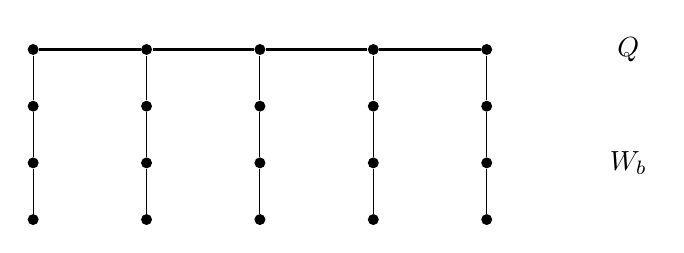
\begin{tikzpicture}[scale=0.9,every node/.style={circle,fill,inner sep=1.4pt}]
\foreach \i in {0,...,4}{ \node (q\i) at (1.6*\i,0) {}; }
\foreach \i in {0,...,3}{ \pgfmathtruncatemacro{\j}{\i+1} \draw[very thick] (q\i)--(q\j); }
\foreach \i in {0,...,4}{
  \node (a\i) at (1.6*\i,-0.8) {}; \node (b\i) at (1.6*\i,-1.6) {}; \node (c\i) at (1.6*\i,-2.4) {};
  \draw (q\i)--(a\i)--(b\i)--(c\i);}
\node[draw=none,fill=none] at (8.4,0) {$Q$};
\node[draw=none,fill=none] at (8.4,-1.6) {$W_b$};
\end{tikzpicture}
\caption{The comb used at the end of the proof: a geodesic $Q$ of the core $K$ with the pendant paths $W_b$ ($b\in Q$) attached. Here $|Q|=5$ and $m=3$.}\label{fig:comb}
\end{figure}

\begin{proof}[Proof of Theorem~\ref{thm:rooted}]
Let $K=F-\bigcup_{b\in B}W_b$. By Lemma~\ref{lem:prop}(i) and (iii), the sets $W_b$ are pairwise disjoint and disjoint from $B$, so $B\subseteq V(K)$. $K$ is connected: a geodesic of $F$ between two vertices of $K$ cannot enter any $W_b$, since it would have to leave through $b$ again. For $b\in B$ and $b'\ne b$, the vertex $b$ has no neighbour in $W_{b'}$: the only vertex outside $W_{b'}$ adjacent to $W_{b'}$ is $b'$, and $b\notin W_{b'}$ by Lemma~\ref{lem:prop}(i). Hence $N_K(b)=N_F(b)\setminus W_b\subseteq B$ by Lemma~\ref{lem:prop}(iv). Since $x\in B$ and $K$ is connected, $B=V(K)$. Thus $F$ consists of the connected graph $K$ together with a pendant path $W_b$ of length $m$ at every vertex $b$ of $K$.

Let $c$ be a centre of $K$. Every vertex of $K$ is within $\rad(K)$ of $c$, and every vertex of $W_b$ is within $d_K(c,b)+m\le\rad(K)+m$. So $\rad(F)\le\rad(K)+m$, and $\diam(K)\ge\rad(K)\ge k+1-m=t$.

Let $Q$ be a geodesic of $K$ with $\diam(K)+1\ge t+1$ vertices. Then $Q\cup\bigcup_{b\in Q}W_b$ is an induced tree of $F$ (Figure~\ref{fig:comb}). Indeed, $Q$ is an induced path of $K=F[V(K)]$, and each $W_b$ is attached only at $b$. Using $k+1=t+m$, its order is
\[
|Q|(m+1)\ \ge\ (t+1)(m+1)\ =\ 2(t+m)+(t-1)(m-1)\ \ge\ 2k+2 .
\]
This contradicts $\tr(F)\le2k+1$ (Lemma~\ref{lem:unroot}). Hence no counterexample exists.
\end{proof}

%======================================================================
\section{Proofs of the main results}\label{sec:main}
%======================================================================

\begin{proof}[Proof of Theorem~\ref{thm:cut}]
Let $c$ be a cut vertex and $r=\rad(G)$. List the components of $G-c$ by decreasing depth $e_1\ge e_2\ge\cdots$, where the depth of a component $A$ is $\max_{a\in A}d(c,a)\ge1$. Then $e_1=\ecc(c)\ge r$. Geodesics from $c$ into the two deepest components form an induced path on $e_1+e_2+1$ vertices. So we may assume $e_1+e_2+1\le 2r-1$, which gives $m:=e_2\le r-2$ and hence $r\ge3$.

Let $A_1,A_2$ be the two deepest components, let $H=G[A_1\cup\{c\}]$, and let $q$ be a geodesic of length $m$ from $c$ into $A_2$. Put $F=G[V(H)\cup V(q)]\cong H\plus_c P_m$. By Lemma~\ref{lem:sep}(a), for $z\in A_1\cup\{c\}$,
\[
\ecc_F(z)=\max\{\ecc_H(z),d(z,c)+e_2\}=\ecc_G(z)\ge r,
\]
while the vertices of $q$ other than $c$ have eccentricity at least $e_1+1\ge r+1$ in $F$. Hence $\rad(F)\ge r$.

Set $k=r-1$ and $t=r-m$, so that $2\le t\le k$ and $m=k-t+1$. By Lemma~\ref{lem:pendant}, $c$ is $(k,t)$-far in $H$, and Theorem~\ref{thm:rooted} applies to $(H,c,k,t)$. If (T) holds, then $\tr(G)\ge\tr(H)\ge 2k+2=2r$. If (R) holds, an induced tree $T\ni c$ of $H$ with $|T|\ge k+t+1=2r-m$, together with $V(q)$, is an induced tree of $G$ on at least $2r$ vertices (Lemma~\ref{lem:sep}(b)).
\end{proof}

\begin{proof}[Proof of Theorem~\ref{thm:84}]
Let $G$ be connected with $\delta(G)\ge1$; so $|V(G)|\ge2$ and $\rad(G)\ge1$.

If $\delta(G)\ge2$, a diametral geodesic is an induced path on $\diam(G)+1$ vertices. Hence $\tr(G)\ge\rad(G)+1>\rad(G)\ge 2\rad(G)/\delta(G)$.

Let $\delta(G)=1$. If $G=K_2$, then $\tr(G)=2=2\rad(G)$. Otherwise the neighbour of a vertex of degree one is a cut vertex, and Theorem~\ref{thm:cut} gives $\tr(G)\ge2\rad(G)=2\rad(G)/\delta(G)$.

Finally, the path on $2r$ vertices has $\delta=1$, radius $r$ and $\tr=2r$, so equality holds.
\end{proof}

\begin{proof}[Proof of Corollary~\ref{cor:2conn}]
A connected graph with at least three vertices that is not $2$-connected has a cut vertex. By Theorem~\ref{thm:cut} it then has $\tr(G)\ge2\rad(G)>2\rad(G)-1$.
\end{proof}

\begin{remark}
In the leaf case one can also go directly through Remark~\ref{rem:leaf}. If $u$ is a leaf with neighbour $w$ and $r=\rad(G)\ge2$, then Theorem~\ref{thm:rooted} with $k=t=r-1$, applied to $(G-u,w)$, gives either an induced tree on $2r$ vertices or a $w$-coherent tree on $2r-1$ vertices. In the second case adding $u$ gives a tree on $2r$ vertices.
\end{remark}

%======================================================================
\section{Computational verification}\label{sec:comp}
%======================================================================

The proofs above are complete and do not depend on computation. We nevertheless tested every statement, and every auxiliary step, by computer. All programs are listed in Appendix~\ref{app:code}. Graphs were generated with \texttt{geng} from \texttt{nauty}~\cite{MP14}.

\paragraph{Exhaustive check of Theorems~\ref{thm:rooted} and~\ref{thm:cut}.} The program \texttt{tlemD.c} reads graphs in graph6 format. For each graph it computes all distances and enumerates all vertex subsets with bit masks to find every induced tree. From these it obtains $\tr(G)$ and, for every vertex $x$, the largest order of an $x$-coherent induced tree. For every $k\ge1$ and every $x$ with $t=\min\{k,d(x,\C_k(G))\}\ge1$ (the strongest admissible $t$), it checks (T) or (R). It also checks $\tr(G)\ge2\rad(G)$ for every graph with a cut vertex and for every graph with a leaf. Table~\ref{tab:exh} summarises the results; there were no failures.

\begin{table}[h]
\centering
\begin{tabular}{rrrrr}
\toprule
$n$ & connected graphs & rooted instances & graphs with a cut vertex & graphs with a leaf\\
\midrule
2 & 1 & 0 & 0 & 1\\
3 & 2 & 2 & 1 & 1\\
4 & 6 & 18 & 3 & 3\\
5 & 21 & 104 & 11 & 10\\
6 & 112 & 811 & 56 & 51\\
7 & 853 & 7\,800 & 385 & 346\\
8 & 11\,117 & 119\,181 & 3\,994 & 3\,675\\
9 & 261\,080 & 3\,102\,468 & 67\,014 & 63\,308\\
10 & 11\,716\,571 & 150\,207\,466 & 1\,973\,029 & 1\,908\,362\\
\midrule
total & 11\,989\,763 & 153\,437\,850 & 2\,044\,493 & 1\,975\,757\\
\bottomrule
\end{tabular}
\caption{Exhaustive verification. Every rooted instance satisfies (T) or (R), and every graph with a cut vertex satisfies $\tr(G)\ge2\rad(G)$.}\label{tab:exh}
\end{table}

\paragraph{Independent re-implementation.} \texttt{crosscheck.py} recomputes the same quantities with \texttt{networkx}, sharing no code with \texttt{tlemD.c}. For $3\le n\le 8$ it reports exactly the instance counts of Table~\ref{tab:exh} (2, 18, 104, 811, 7\,800, 119\,181) and no failures.

\paragraph{Eleven vertices.} A third checker, \texttt{lemd3.c}, was written independently of the other two during an audit of the proof. It enumerates induced trees by a leaf-deletion recursion over vertex subsets. For every rooted instance and every admissible $t$ (not only the largest), it tests (T) or (R), and it tests Theorem~\ref{thm:cut}. It skips only instances that are settled outright:
\begin{itemize}
\item those where a diametral path gives (T);
\item those where a geodesic from $x$ gives (R);
\item graphs of diameter at most $2$. In such a graph only $k=t=1$ is admissible, and that case is settled by a geodesic from $x$. A cut vertex then forces radius $1$.
\end{itemize}
Run on all $1\,006\,700\,565$ connected graphs with $11$ vertices (split as \verb|geng -cq 11 r/4|, $r=0,\dots,3$), it tested $693\,086\,400$ non-trivial rooted instances and all $105\,442\,877$ graphs that have a cut vertex and diameter at least $3$. There was no failure. (Graphs with a cut vertex and diameter at most $2$ have a dominating vertex, so Theorem~\ref{thm:cut} is trivial for them.) We re-ran \texttt{lemd3.c} ourselves on $n=8,9$; again there was no failure. With the diameter-$2$ shortcut switched off (argument \texttt{2}), it reports for $n=9$ the same number $67\,014$ of graphs with a cut vertex as Table~\ref{tab:exh}.

\paragraph{Random graphs.} We fed \texttt{tlemD.c} with $12\,000$ random graphs $G(15,p)$ with $p$ equal to $0.12$, $0.16$, $0.20$ or $0.25$, generated by \texttt{genrang} (disconnected ones were skipped), and with $6\,000$ sparse graphs on $10$ to $16$ vertices produced by \texttt{gen\_sparse.py} (random trees plus a few random edges). In total $10\,687$ connected graphs and $486\,271$ rooted instances were checked, with no failures. A further $600$ sparse connected graphs with $17$ to $20$ vertices (\texttt{gen\_sparse2.py}, checked by \texttt{tlemDr} compiled with \texttt{MAXN} raised to $22$) gave $55\,205$ rooted instances and $598$ graphs with a cut vertex, again with no failure.

\paragraph{Auxiliary steps.} \texttt{sublemmas.py} tested, on $8\,000$ random connected graphs with $4$ to $22$ vertices, the following claims: the equivalence of Lemma~\ref{lem:pendant} ($164\,902$ instances); the preservation of farness in Lemma~\ref{lem:nbrs}(a) ($52\,158$); farness in Lemma~\ref{lem:noncut} ($3\,001$); connectivity in Lemma~\ref{lem:farthest} ($6\,081$); the inequality $\mu\ge m$ of Lemma~\ref{lem:nbrs}(d) ($2\,729$); and farness in $\tilde G$ in Lemma~\ref{lem:nbrs}(e) ($3\,803$). No violation occurred.

%======================================================================
\section{Open problems}\label{sec:open}
%======================================================================

\begin{conjecture}[Path version]\label{conj:path}
Under the hypotheses of Theorem~\ref{thm:rooted}, either $\tr(G)\ge2k+2$, or $x$ is an end of an induced path on at least $k+t+1$ vertices.
\end{conjecture}

Conjecture~\ref{conj:path} would imply both Theorem~\ref{thm:rooted} and the Bacs\'o--Tuza lemma. The program \texttt{tbt.c} confirms it for all connected graphs with at most $10$ vertices: $156\,575\,328$ instances $(G,x,k,t)$ over all admissible $t$, with no failure. Our proof does not adapt directly, because the unrooting equivalence (Lemma~\ref{lem:unroot}) fails for paths.

\begin{conjecture}\label{conj:sc}
If $G$ is connected and $\diam(G)>\rad(G)$, then $\tr(G)\ge2\rad(G)$.
\end{conjecture}

Every graph with a leaf satisfies $\diam>\rad$, so Conjecture~\ref{conj:sc} would contain the leaf case of Theorem~\ref{thm:cut}. The program \texttt{tdiam.c} confirms it for all $8\,052\,809$ connected graphs with at most $10$ vertices and $\diam>\rad$. The analogous statement for induced paths fails: the graph $C_4\circ K_1$ of Remark~\ref{rem:nopath} (graph6 code \verb|G?`FE_|) is a counterexample. Corollary~\ref{cor:2conn} and Conjecture~\ref{conj:sc} suggest the following question. \emph{Which $2$-connected self-centred graphs attain the Erd\H{o}s--Saks--S\'os bound $\tr(G)=2\rad(G)-1$?} Even cycles and the cocktail-party graphs $K_{2,2,\dots,2}$ (with at least two parts) do.

\paragraph{Acknowledgement of methods.} The reductions in Lemma~\ref{lem:nbrs}(a)--(d) follow the structure of the Bacs\'o--Tuza induction~\cite{BT90}, as formalised in~\cite{Mak}. The coherent-root formulation, the cut-root reduction (Lemma~\ref{lem:noncut}), the unrooting equivalence (Lemma~\ref{lem:unroot}) and the sibling propagation (Lemmas~\ref{lem:sibling} and~\ref{lem:prop}) are new as far as we know.

\begin{thebibliography}{99}
\bibitem{BT90} G.~Bacs\'o and Zs.~Tuza, A characterization of graphs without long induced paths, \emph{J. Graph Theory} 14 (1990), 455--464.
\bibitem{DeL05} E.~DeLaVi\~na, Graffiti.pc: a variant of Graffiti, in: \emph{Graphs and Discovery}, DIMACS Ser. Discrete Math. Theoret. Comput. Sci. 69, Amer. Math. Soc., 2005, 71--79.
\bibitem{WOWII} E.~DeLaVi\~na, \emph{Written on the Wall II: Conjectures of Graffiti.pc}, \url{http://cms.uhd.edu/faculty/delavinae/research/wowII/all.html} (Conjecture~84).
\bibitem{ESS86} P.~Erd\H{o}s, M.~Saks and V.~T.~S\'os, Maximum induced trees in graphs, \emph{J. Combin. Theory Ser. B} 41 (1986), 61--79.
\bibitem{FC} Google DeepMind, \emph{Formal Conjectures}, file \nolinkurl{FormalConjectures/WrittenOnTheWallII/GraphConjecture84.lean}, \url{https://github.com/google-deepmind/formal-conjectures} (state of 23 October 2026).
\bibitem{Fer26} A.~Ferudun, Three Graffiti.pc conjectures on largest induced trees: proofs of Conjectures 141, 142, and 143, arXiv:2608.01396 (2026).
\bibitem{FLS09} J.~Fox, P.-S.~Loh and B.~Sudakov, Large induced trees in $K_r$-free graphs, \emph{J. Combin. Theory Ser. B} 99 (2009), 494--501.
\bibitem{Mak} C.~Maki, \emph{WOW II \#144 in Lean 4} (formal proof including a formalisation of the Bacs\'o--Tuza Induced Path Lemma), \url{https://github.com/beowulf127/wowii144-lean} (2026).
\bibitem{MP14} B.~D.~McKay and A.~Piperno, Practical graph isomorphism, II, \emph{J. Symbolic Comput.} 60 (2014), 94--112.
\end{thebibliography}

\appendix
%======================================================================
\section{Source code}\label{app:code}
%======================================================================

The C programs read connected graphs in graph6 format from standard input, for example \verb+geng -cq 10 | ./tlemD+. The $n=10$ run of \texttt{tlemD} was split as \verb|geng -cq 10 r/4| for $r=0,1,2,3$, and the $n=10$ runs of \texttt{tbt} and \texttt{tdiam} as \verb|geng -cq 10 r/2| for $r=0,1$. They were compiled with \verb|gcc -O2|. The variant \texttt{tlemDr} used for random graphs is \texttt{tlemD.c} with an added connectivity filter: the call \verb|parse_g6(line); cnt++;| is replaced by \verb|parse_g6(line); if(!conn((1u<<n)-1)) continue; cnt++;|. The random input was produced by
\begin{verbatim}
(for p in 12 16 20 25; do genrang -g -P$p/100 15 3000; done; \
 python3 gen_sparse.py 7 16 6000) | ./tlemDr
\end{verbatim}

\subsection{\texttt{tlemD.c}: exhaustive check of Theorems~\ref{thm:rooted} and~\ref{thm:cut}}
\begin{lstlisting}[language=C]
// Exhaustive check of Lemma D: G connected, k>=1, x with t*=min(dist(x,C_k),k)>=1:
//   (T) tree(G)>=2k+2  or  (R0) exists induced tree T containing x, |T|>=k+t*+1, N_T(x) inside one component of G-x.
// Also checks the cut-vertex corollary: G has a cut vertex => tree(G) >= 2 rad(G); and leaf corollary.
#include <stdio.h>
#include <stdlib.h>
#include <string.h>
#define MAXN 16
static int n; static unsigned adj[MAXN];
static int popc(unsigned x){return __builtin_popcount(x);}
static void parse_g6(const char*s){ int k=0; n=s[k++]-63; memset(adj,0,sizeof adj); int bits=0; unsigned char c=0;
  for(int j=1;j<n;j++) for(int i=0;i<j;i++){ if(bits==0){c=s[k++]-63; bits=6;} bits--; if((c>>bits)&1){adj[i]|=1u<<j; adj[j]|=1u<<i;} } }
static int conn(unsigned S){ if(!S) return 0; unsigned seen=S&-S, fr=seen; while(fr){ unsigned nf=0; for(unsigned t=fr;t;t&=t-1){int v=__builtin_ctz(t); nf|=adj[v]&S;} nf&=~seen; seen|=nf; fr=nf;} return seen==S; }
static unsigned comp(unsigned S, int v){ unsigned seen=1u<<v, fr=seen; while(fr){ unsigned nf=0; for(unsigned t=fr;t;t&=t-1){int w=__builtin_ctz(t); nf|=adj[w]&S;} nf&=~seen; seen|=nf; fr=nf;} return seen; }
static int edges_in(unsigned S){ int e=0; for(unsigned t=S;t;t&=t-1){int v=__builtin_ctz(t); e+=popc(adj[v]&S);} return e/2; }
static int D[MAXN][MAXN];
static void bfs_all(){ for(int s=0;s<n;s++){ for(int i=0;i<n;i++) D[s][i]=99; D[s][s]=0; unsigned fr=1u<<s, seen=fr; int d=0; while(fr){ d++; unsigned nf=0; for(unsigned t=fr;t;t&=t-1){int v=__builtin_ctz(t); nf|=adj[v];} nf&=~seen; for(unsigned t=nf;t;t&=t-1) D[s][__builtin_ctz(t)]=d; seen|=nf; fr=nf; } } }
int main(){ char line[256]; long cnt=0, cases=0, failD=0, cutg=0, failcut=0, leafg=0, failleaf=0; static unsigned char istree[1<<MAXN];
  while(fgets(line,sizeof line,stdin)){ line[strcspn(line,"\n")]=0; parse_g6(line); cnt++; unsigned full=(1u<<n)-1;
    bfs_all(); int ecc[MAXN], rad=99; for(int v=0;v<n;v++){int e=0; for(int w=0;w<n;w++) if(D[v][w]>e) e=D[v][w]; ecc[v]=e; if(e<rad) rad=e;}
    int tsz=0; for(unsigned S=1;S<=full;S++){ int kk=popc(S); istree[S]=(kk==1)||(edges_in(S)==kk-1 && conn(S)); if(istree[S]&&kk>tsz) tsz=kk; }
    // rho0[x]
    int rho0[MAXN]; for(int x=0;x<n;x++){ unsigned rest=full&~(1u<<x); unsigned cm[MAXN]; int nc=0; unsigned left=rest; while(left){ int v=__builtin_ctz(left); unsigned c=comp(rest,v); cm[nc++]=c; left&=~c; }
      int best=1; for(unsigned S=1;S<=full;S++){ if(!((S>>x)&1)||!istree[S]) continue; int p=popc(S); if(p<=best) continue; unsigned nb=adj[x]&S; int ok=(nb==0); for(int i=0;i<nc&&!ok;i++) if((nb&~cm[i])==0) ok=1; if(ok) best=p; } rho0[x]=best; }
    for(int k=1;k<n;k++) for(int x=0;x<n;x++){ int dk=99; for(int y=0;y<n;y++) if(ecc[y]<=k && D[x][y]<dk) dk=D[x][y]; int t=dk<k?dk:k; if(t<1) continue; cases++;
      if(tsz>=2*k+2) continue; if(rho0[x]>=k+t+1) continue; failD++; if(failD<=10) printf("FAIL-D %s k=%d t=%d x=%d\n",line,k,t,x); }
    int hascut=0; for(int v=0;v<n&&!hascut;v++) if(n>=3 && !conn(full&~(1u<<v))) hascut=1;
    if(hascut){ cutg++; if(tsz<2*rad){ failcut++; printf("FAIL-CUT %s\n",line);} }
    int hasleaf=0; for(int v=0;v<n;v++) if(popc(adj[v])==1) hasleaf=1;
    if(hasleaf){ leafg++; if(tsz<2*rad){ failleaf++; printf("FAIL-LEAF %s\n",line);} }
  }
  printf("graphs %ld lemmaD-cases %ld failD %ld | cutgraphs %ld failcut %ld | leafgraphs %ld failleaf %ld\n",cnt,cases,failD,cutg,failcut,leafg,failleaf); }
\end{lstlisting}

\subsection{\texttt{crosscheck.py}: independent re-implementation}
\begin{lstlisting}[language=Python]
# Independent (networkx-based) re-implementation of the Lemma D check, for cross-validation on small orders.
import sys, itertools, networkx as nx
def is_induced_tree(G, S):
    H = G.subgraph(S)
    return len(S) >= 1 and nx.is_tree(H)
def check(G):
    V = list(G); n = len(V)
    E = nx.eccentricity(G)
    trees = [frozenset(S) for r in range(1, n+1) for S in itertools.combinations(V, r) if is_induced_tree(G, S)]
    tsz = max(len(S) for S in trees)
    bad = 0; cases = 0
    for x in V:
        Gx = G.copy(); Gx.remove_node(x)
        comps = [set(c) for c in nx.connected_components(Gx)]
        rho = max(len(S) for S in trees if x in S and (not set(G[x]) & S or any(set(G[x]) & S <= c for c in comps)))
        D = nx.single_source_shortest_path_length(G, x)
        for k in range(1, n):
            C = [z for z in V if E[z] <= k]
            t = min([D[z] for z in C], default=10**9); t = min(t, k)
            if t < 1: continue
            cases += 1
            if not (tsz >= 2*k+2 or rho >= k+t+1): bad += 1
    rad = min(E.values())
    cut = n >= 3 and len(list(nx.articulation_points(G))) > 0
    return cases, bad, (cut and tsz < 2*rad)
tot = [0,0,0,0]
for line in sys.stdin:
    G = nx.from_graph6_bytes(line.strip().encode())
    c, b, cf = check(G)
    tot[0] += 1; tot[1] += c; tot[2] += b; tot[3] += cf
print("graphs %d cases %d failD %d failcut %d" % tuple(tot))
\end{lstlisting}

\subsection{\texttt{sublemmas.py}: randomized checks of the auxiliary steps}
Run as \verb|python3 sublemmas.py 1| and \verb|python3 sublemmas.py 2|.
\begin{lstlisting}[language=Python]
# Randomized sanity checks of the auxiliary facts used in the proof of Lemma D.
import random, networkx as nx, itertools, sys
random.seed(int(sys.argv[1]) if len(sys.argv)>1 else 1)

def ecc_all(G):
    return nx.eccentricity(G)

def Ck(G, k, E=None):
    E = E or ecc_all(G)
    return {v for v in G if E[v] <= k}

def far(G, x, k, t):
    D = nx.single_source_shortest_path_length(G, x)
    return all(D[z] >= t for z in Ck(G, k))

def add_pendant(G, v, m, tag):
    H = G.copy(); prev = v
    for h in range(1, m+1):
        H.add_edge(prev, (tag, h)); prev = (tag, h)
    return H

def rand_conn(n, p):
    while True:
        G = nx.gnp_random_graph(n, p)
        if nx.is_connected(G): return G

bad = {'equiv':0,'caseA':0,'P2':0,'P3d':0,'P3e':0,'Gu':0}
cnt = {k:0 for k in bad}
for it in range(4000):
    n = random.randint(4, 22); p = random.choice([0.08,0.12,0.18,0.25,0.35])
    G = rand_conn(n, p)
    E = ecc_all(G); rad = min(E.values())
    x = random.choice(list(G))
    # 1. Equivalence lemma
    for k in range(1, max(E.values())+2):
        for t in range(1, k+1):
            m = k - t + 1
            Hp = add_pendant(G, x, m, 'P')
            lhs = min(ecc_all(Hp).values()) >= k+1
            rhs = far(G, x, k, t)
            cnt['equiv'] += 1
            if lhs != rhs: bad['equiv'] += 1
    # 2. Case A: s ~ x non-cut, x far in G (t<=k) => x far in G-s
    for k in range(1, max(E.values())+1):
        Dx = nx.single_source_shortest_path_length(G, x)
        C = Ck(G, k, E); tstar = min([Dx[z] for z in C], default=10**9); tstar = min(tstar, k)
        for t in range(1, tstar+1):
            for s in G[x]:
                Gs = G.copy(); Gs.remove_node(s)
                if not nx.is_connected(Gs): continue
                cnt['caseA'] += 1
                if not far(Gs, x, k, t): bad['caseA'] += 1
    # 3. P2: x cut vertex, far by t; e' <= k-1 => far by tau in G1
    if x in set(nx.articulation_points(G)):
        Gx = G.copy(); Gx.remove_node(x); comps = list(nx.connected_components(Gx))
        Dx = nx.single_source_shortest_path_length(G, x)
        depth = [max(Dx[v] for v in c) for c in comps]
        i1 = max(range(len(comps)), key=lambda i: depth[i]); e1 = depth[i1]
        ep = max(depth[i] for i in range(len(comps)) if i != i1)
        G1 = G.subgraph(set(comps[i1]) | {x}).copy()
        for k in range(1, e1):
            if e1 + ep + 1 >= 2*k+2: continue
            C = Ck(G, k, E); tstar = min([Dx[z] for z in C], default=10**9); tstar=min(tstar,k)
            for t in range(1, tstar+1):
                tau = min(t, k+1-ep)
                cnt['P2'] += 1
                if not (1 <= tau <= k and far(G1, x, k, tau)): bad['P2'] += 1
    # 4/5. P3: s neighbor of x, s cut vertex; U, u farthest; G-u connected; if x not far in G-u => mu >= k-t+1;
    #       G~ = G[X+s+q]: x far in G~ provided e_X >= k+1 and mu <= k-1 ... (we test the implication used)
    Dx = nx.single_source_shortest_path_length(G, x)
    for s in G[x]:
        Gs = G.copy(); Gs.remove_node(s)
        if nx.is_connected(Gs): continue
        X = nx.node_connected_component(Gs, x); U = set(G) - X - {s}
        Ds = nx.single_source_shortest_path_length(G, s)
        mu = max(Ds[v] for v in U); u = max(U, key=lambda v: Ds[v])
        Gu = G.copy(); Gu.remove_node(u)
        cnt['Gu'] += 1
        if not nx.is_connected(Gu): bad['Gu'] += 1; continue
        for k in range(1, max(E.values())+1):
            C = Ck(G, k, E); tstar = min([Dx[z] for z in C], default=10**9); tstar=min(tstar,k)
            for t in range(2, tstar+1):
                if not far(Gu, x, k, t):
                    cnt['P3d'] += 1
                    if mu < k-t+1: bad['P3d'] += 1
                # P3e: if mu <= k-1 (so e_X >= k+1 automatically), x far in G~
                if mu <= k-1:
                    path = nx.shortest_path(G, s, u)
                    Gt = G.subgraph(X | {s} | set(path)).copy()
                    cnt['P3e'] += 1
                    if not far(Gt, x, k, t): bad['P3e'] += 1
print('checked', cnt)
print('violations', bad)
\end{lstlisting}

\subsection{\texttt{gen\_sparse.py}: random sparse connected graphs}
\begin{lstlisting}[language=Python]
import random, sys, networkx as nx
random.seed(int(sys.argv[1])); N=int(sys.argv[2]); cnt=int(sys.argv[3])
out=[]
for _ in range(cnt):
    n=random.randint(10,N)
    T=nx.random_labeled_tree(n) if hasattr(nx,'random_labeled_tree') else nx.random_tree(n)
    G=nx.Graph(T)
    extra=random.choice([0,1,2,3,4,5,6,8,10])
    nodes=list(G)
    for _ in range(extra):
        a,b=random.sample(nodes,2); G.add_edge(a,b)
    out.append(nx.to_graph6_bytes(G,header=False).decode().strip())
print("\n".join(out))
\end{lstlisting}

\subsection{\texorpdfstring{\texttt{lemd3.c}: independent checker used for $n=11$}{lemd3.c: independent checker used for n=11}}
\begin{lstlisting}[language=C]
/* Exhaustive check of Lemma D and Theorem A on graphs read in graph6 from stdin.
   Lemma D: G connected, k>=1, 1<=t<=k, x t-far wrt k  =>  tree(G)>=2k+2  or
            exists induced tree T containing x, |T|>=k+t+1, N_T(x) inside one component of G-x.
   Theorem A: G connected with a cut vertex => tree(G) >= 2 rad(G).
   Also records tightness statistics. */
#include <stdio.h>
#include <stdlib.h>
#include <string.h>
#define MAXN 24
static int n;
static unsigned adj[MAXN];
static int dist[MAXN][MAXN], ecc[MAXN];
static unsigned char *istree;
static long long nskipped=0, ngraphs=0, ninst=0, nfailD=0, nfailA=0, ncut=0, tightA=0, tightD=0;

static int parse_g6(const char *s){
  const unsigned char *p=(const unsigned char*)s;
  if(p[0]=='>' ) { while(*p && *p!='<') p++; p+=2; }
  int nn=p[0]-63; p++;
  memset(adj,0,sizeof adj);
  int x=0,bits=0;
  for(int j=1;j<nn;j++) for(int i=0;i<j;i++){
    if(bits==0){ x=*p++-63; bits=6; }
    bits--;
    if((x>>bits)&1){ adj[i]|=1u<<j; adj[j]|=1u<<i; }
  }
  return nn;
}
static void bfs_all(void){
  for(int s=0;s<n;s++){
    for(int v=0;v<n;v++) dist[s][v]=-1;
    unsigned seen=1u<<s, fr=1u<<s; int d=0; dist[s][s]=0;
    while(fr){ unsigned nf=0; for(int v=0;v<n;v++) if(fr>>v&1) nf|=adj[v]; nf&=~seen; d++;
      for(int v=0;v<n;v++) if(nf>>v&1) dist[s][v]=d; seen|=nf; fr=nf; }
    ecc[s]=0; for(int v=0;v<n;v++){ if(dist[s][v]<0){ecc[s]=1000;} else if(dist[s][v]>ecc[s]) ecc[s]=dist[s][v]; }
  }
}
static unsigned reach(unsigned start, unsigned allowed){ /* component of start within allowed */
  unsigned seen=start, fr=start;
  while(fr){ unsigned nf=0; for(int v=0;v<n;v++) if(fr>>v&1) nf|=adj[v]; nf&=allowed&~seen; seen|=nf; fr=nf; }
  return seen;
}
int main(int argc,char**argv){
  char line[512];
  int verbose = argc>1 ? atoi(argv[1]) : 0;
  istree = malloc(1u<<MAXN);
  while(fgets(line,sizeof line,stdin)){
    n=parse_g6(line); ngraphs++;
    { unsigned allm=(1u<<n)-1; int d2=1; for(int u=0;u<n && d2;u++){ unsigned r=adj[u]|(1u<<u); unsigned T=adj[u]; while(T){int v=__builtin_ctz(T); T&=T-1; r|=adj[v];} if(r!=allm) d2=0; } if(d2 && !(verbose&2)) continue; }
    bfs_all();
    int diam=0, rad=1000; for(int v=0;v<n;v++){ if(ecc[v]>diam) diam=ecc[v]; if(ecc[v]<rad) rad=ecc[v]; }
    if(diam>=1000) continue; /* disconnected */
    unsigned all=(n==32)?0xffffffffu:((1u<<n)-1);
    /* cut vertex? */
    int hascut=0;
    for(int v=0;v<n && !hascut;v++){ unsigned rest=all&~(1u<<v); if(!rest) continue; int s=__builtin_ctz(rest);
      if(reach(1u<<s,rest)!=rest) hascut=1; }
    if(diam<=2 && !(verbose&2)) { if(hascut) ncut++; continue; } /* see note: diam<=2 => only k=1,t=1 (trivial) and cut=>rad=1 */
    /* quick filter: is any Lemma D instance or the Theorem A check non-trivial? */
    { int need = (hascut && diam+1<2*rad);
      for(int k=1;k<diam && !need;k++){ if(diam>=2*k+1) continue;
        unsigned Ck=0; for(int z=0;z<n;z++) if(ecc[z]<=k) Ck|=1u<<z;
        for(int x=0;x<n && !need;x++){ if(ecc[x]<=k) continue;
          int f=1000; for(int z=0;z<n;z++) if(Ck>>z&1) if(dist[x][z]<f) f=dist[x][z];
          int tmax=f<k?f:k; if(tmax<1) continue;
          if(ecc[x] < k+tmax) need=1; } }
      if(!need){ if(hascut) ncut++; nskipped++; continue; } }
    /* induced trees DP */
    unsigned N=1u<<n; int maxtree=0; int maxR[MAXN]; for(int v=0;v<n;v++) maxR[v]=0;
    /* components of G-x */
    unsigned comp[MAXN][MAXN]; int ncomp[MAXN];
    for(int x=0;x<n;x++){ unsigned rest=all&~(1u<<x); ncomp[x]=0;
      while(rest){ unsigned c=reach(rest&(-rest),all&~(1u<<x)); comp[x][ncomp[x]++]=c; rest&=~c; } }
    istree[0]=0;
    for(unsigned S=1;S<N;S++){
      int sz=__builtin_popcount(S);
      if(sz==1){ istree[S]=1; }
      else { int leaf=-1; unsigned T=S; while(T){ int v=__builtin_ctz(T); T&=T-1; if(__builtin_popcount(adj[v]&S)==1){leaf=v;break;} }
        istree[S]= (leaf>=0) ? istree[S^(1u<<leaf)] : 0; }
      if(!istree[S]) continue;
      if(sz>maxtree) maxtree=sz;
      unsigned T=S; while(T){ int x=__builtin_ctz(T); T&=T-1; if(sz<=maxR[x]) continue;
        unsigned nb=adj[x]&S; int ok=0; if(!nb) ok=1; else for(int c=0;c<ncomp[x];c++) if((nb&~comp[x][c])==0){ok=1;break;}
        if(ok) maxR[x]=sz; }
    }
    if(hascut){ ncut++; if(maxtree<2*rad){ nfailA++; printf("FAIL_A %s",line);} else if(maxtree==2*rad) tightA++; }
    for(int k=1;k<diam;k++){
      unsigned Ck=0; for(int z=0;z<n;z++) if(ecc[z]<=k) Ck|=1u<<z;
      for(int x=0;x<n;x++){ if(ecc[x]<=k) continue;
        int f=1000; for(int z=0;z<n;z++) if(Ck>>z&1) if(dist[x][z]<f) f=dist[x][z];
        int tmax = f<k? f : k; if(tmax<1) continue;
        for(int t=1;t<=tmax;t++){ ninst++;
          int T_ok = maxtree>=2*k+2, R_ok = maxR[x]>=k+t+1;
          if(!T_ok && !R_ok){ nfailD++; printf("FAIL_D k=%d t=%d x=%d %s",k,t,x,line); }
          else if(!T_ok && maxR[x]==k+t+1 && t>=2) { tightD++; if(verbose&1) printf("TIGHT_D k=%d t=%d x=%d %s",k,t,x,line);} }
      }
    }
  }
  fprintf(stderr,"skippedTrivial=%lld graphs=%lld cutgraphs=%lld instances(D)=%lld failD=%lld failA=%lld tightA=%lld tightD(t>=2)=%lld\n",
          nskipped,ngraphs,ncut,ninst,nfailD,nfailA,tightA,tightD);
  return 0;
}
\end{lstlisting}

\subsection{\texttt{gen\_sparse2.py}: larger sparse graphs}
Run as \verb+python3 gen_sparse2.py 11 17 20 600 | ./tlemDr22+.
\begin{lstlisting}[language=Python]
import random, sys, networkx as nx
random.seed(int(sys.argv[1])); lo=int(sys.argv[2]); hi=int(sys.argv[3]); cnt=int(sys.argv[4])
for _ in range(cnt):
    n=random.randint(lo,hi)
    G=nx.Graph(nx.random_labeled_tree(n) if hasattr(nx,'random_labeled_tree') else nx.random_tree(n))
    for _ in range(random.choice([1,2,3,4,5,6,8])):
        a,b=random.sample(list(G),2); G.add_edge(a,b)
    print(nx.to_graph6_bytes(G,header=False).decode().strip())
\end{lstlisting}

\subsection{\texttt{tbt.c}: evidence for Conjecture~\ref{conj:path}}
\begin{lstlisting}[language=C]
// Test BT-tree: for connected H, k>=1, 1<=t<=k, x with dist(x, kcenter)>=t:
//  (R) x starts induced path with >= k+t edges, or (T) H has induced tree with >= 2k+2 vertices.
// Also record cases where only plain BT unrooted (path >= 2k edges) holds.
#include <stdio.h>
#include <stdlib.h>
#include <string.h>
#define MAXN 16
static int n; static unsigned adj[MAXN];
static int popc(unsigned x){return __builtin_popcount(x);}
static void parse_g6(const char*s){ int k=0; n=s[k++]-63; memset(adj,0,sizeof adj); int bits=0; unsigned char c=0;
  for(int j=1;j<n;j++) for(int i=0;i<j;i++){ if(bits==0){c=s[k++]-63; bits=6;} bits--; if((c>>bits)&1){adj[i]|=1u<<j; adj[j]|=1u<<i;} } }
static int dist[MAXN][MAXN];
static void bfs_all(){ for(int s=0;s<n;s++){ for(int i=0;i<n;i++) dist[s][i]=-1; dist[s][s]=0; unsigned fr=1u<<s, seen=fr; int d=0; while(fr){ d++; unsigned nf=0; for(unsigned t=fr;t;t&=t-1){int v=__builtin_ctz(t); nf|=adj[v];} nf&=~seen; for(unsigned t=nf;t;t&=t-1) dist[s][__builtin_ctz(t)]=d; seen|=nf; fr=nf; } } }
static int conn(unsigned S){ if(!S) return 0; unsigned seen=S&-S, fr=seen; while(fr){ unsigned nf=0; for(unsigned t=fr;t;t&=t-1){int v=__builtin_ctz(t); nf|=adj[v]&S;} nf&=~seen; seen|=nf; fr=nf;} return seen==S; }
static int edges_in(unsigned S){ int e=0; for(unsigned t=S;t;t&=t-1){int v=__builtin_ctz(t); e+=popc(adj[v]&S);} return e/2; }
static int best; static void lip(int v, unsigned S, int len){ if(len>best) best=len; unsigned cand=adj[v]&~S; for(unsigned t=cand;t;t&=t-1){ int x=__builtin_ctz(t); if((adj[x]&S)==(1u<<v)) lip(x,S|(1u<<x),len+1); } }
int main(){ char line[256]; long cnt=0, cases=0, fail=0;
  while(fgets(line,sizeof line,stdin)){ line[strcspn(line,"\n")]=0; parse_g6(line); cnt++; unsigned full=(1u<<n)-1;
    bfs_all(); int ecc[MAXN]; for(int v=0;v<n;v++){int e=0; for(int w=0;w<n;w++) if(dist[v][w]>e) e=dist[v][w]; ecc[v]=e;}
    int tsz=0; for(unsigned S=1;S<=full;S++){ int k=popc(S); if(k<=tsz) continue; if(edges_in(S)==k-1 && conn(S)) tsz=k; }
    int rootlen[MAXN]; for(int x=0;x<n;x++){ best=0; lip(x,1u<<x,1); rootlen[x]=best-1; } // edges
    for(int k=1;k<n;k++){ for(int x=0;x<n;x++){ int dk=99; for(int y=0;y<n;y++) if(ecc[y]<=k && dist[x][y]<dk) dk=dist[x][y];
        int tmax = dk<k?dk:k; for(int t=1;t<=tmax;t++){ cases++; if(rootlen[x]>=k+t) continue; if(tsz>=2*k+2) continue; fail++; if(fail<=5) printf("FAIL %s k=%d t=%d x=%d rootlen=%d tree=%d\n",line,k,t,x,rootlen[x],tsz); } } }
  }
  printf("graphs %ld cases %ld fail %ld\n",cnt,cases,fail); }
\end{lstlisting}

\subsection{\texttt{tdiam.c}: evidence for Conjecture~\ref{conj:sc}}
\begin{lstlisting}[language=C]
#include <stdio.h>
#include <stdlib.h>
#include <string.h>
#define MAXN 16
static int n; static unsigned adj[MAXN];
static int popc(unsigned x){return __builtin_popcount(x);}
static void parse_g6(const char*s){ int k=0; n=s[k++]-63; memset(adj,0,sizeof adj); int bits=0; unsigned char c=0;
  for(int j=1;j<n;j++) for(int i=0;i<j;i++){ if(bits==0){c=s[k++]-63; bits=6;} bits--; if((c>>bits)&1){adj[i]|=1u<<j; adj[j]|=1u<<i;} } }
static int dist[MAXN][MAXN];
static void bfs_all(){ for(int s=0;s<n;s++){ for(int i=0;i<n;i++) dist[s][i]=-1; dist[s][s]=0; unsigned fr=1u<<s, seen=fr; int d=0; while(fr){ d++; unsigned nf=0; for(unsigned t=fr;t;t&=t-1){int v=__builtin_ctz(t); nf|=adj[v];} nf&=~seen; for(unsigned t=nf;t;t&=t-1) dist[s][__builtin_ctz(t)]=d; seen|=nf; fr=nf; } } }
static int conn(unsigned S){ if(!S) return 0; unsigned seen=S&-S, fr=seen; while(fr){ unsigned nf=0; for(unsigned t=fr;t;t&=t-1){int v=__builtin_ctz(t); nf|=adj[v]&S;} nf&=~seen; seen|=nf; fr=nf;} return seen==S; }
static int edges_in(unsigned S){ int e=0; for(unsigned t=S;t;t&=t-1){int v=__builtin_ctz(t); e+=popc(adj[v]&S);} return e/2; }
int main(){ char line[256]; long cnt=0, nsc=0, fail=0, failP=0;
  while(fgets(line,sizeof line,stdin)){ line[strcspn(line,"\n")]=0; parse_g6(line); unsigned full=(1u<<n)-1; cnt++;
    bfs_all(); int rad=99, diam=0; for(int v=0;v<n;v++){int e=0; for(int w=0;w<n;w++) if(dist[v][w]>e) e=dist[v][w]; if(e<rad) rad=e; if(e>diam) diam=e;}
    if(diam==rad) continue; nsc++;
    int tsz=0, psz=0; for(unsigned S=1;S<=full;S++){ int k=popc(S); if(k<=tsz && k<=psz) continue; if(edges_in(S)==k-1 && conn(S)){ if(k>tsz) tsz=k; int ok=1; for(unsigned t=S;t;t&=t-1){int v=__builtin_ctz(t); if(popc(adj[v]&S)>2){ok=0;break;}} if(ok && k>psz) psz=k; } }
    if(tsz<2*rad){ fail++; if(fail<=5) printf("FAIL %s rad=%d diam=%d tree=%d\n",line,rad,diam,tsz);} 
    if(psz<2*rad){ failP++; if(failP<=3) printf("PATHFAIL %s rad=%d diam=%d path=%d tree=%d\n",line,rad,diam,psz,tsz);} }
  printf("graphs %ld non-self-centered %ld: tree<2rad %ld ; path<2rad %ld\n",cnt,nsc,fail,failP); }
\end{lstlisting}

\end{document}
